\chapter{Results}

\section{Experiment 1}
The mean sentence score for each talker across all listeners is given in Figure~\ref{fig:ExpOneBarplot}.  Darker bars represent the original unmodified talkers, while light bars represent resynthesized talkers.  Contrary to expectations, not all resynthesized stimuli are lower than their unmodified counterparts, suggesting that distortion due to the resynthesis process was relatively minimal.  With regard to Research Question~1 — how does prosody relate to intelligibility — a complicated picture emerges.  One explanation for these results is to postulate that Talker~\ac{a}, despite being highly intelligible, does not have especially intelligible prosody, evidenced in particular by the fact that scores for Talker~\ac{ca} are lower than the scores for Talker~\ac{cb}.  On the same grounds, and on the additional observation that scores for Talker~\ac{ab} are greater than for Talker~\ac{ac}, we might conclude that Talker~\ac{b} has more intelligible prosody than the other two talkers.

\begin{figure}[htbp]
	\begin{centering}
	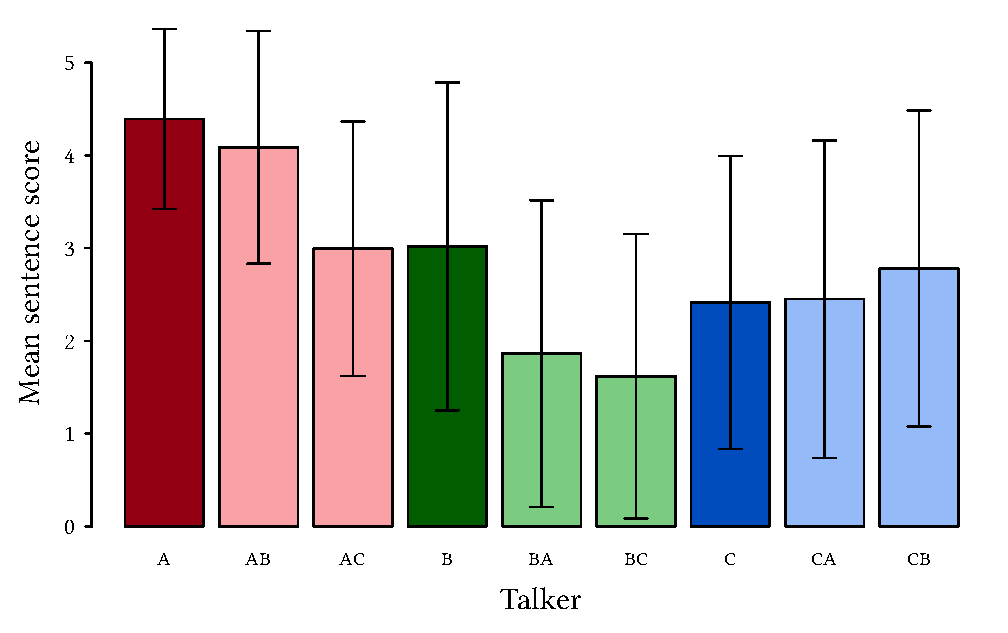
\includegraphics{figures/results/ExpOneBarplot.eps}
	\caption[Barplot of mean sentence scores for Experiment~1]{Barplot of mean sentence scores for Experiment~1.  Error bars are ±1 standard error; lighter colors indicate resynthesized talkers.  See Section~\ref{sec:ExpDesign} for explanation of talker codes.\label{fig:ExpOneBarplot}}
	\end{centering}
\end{figure}

With regard to the question of whether low-intelligibility talkers can be made more intelligible through prosody alone, it would appear that the answer is “yes”: Talker~\ac{cb} appears to have higher scores than Talker~\ac{c}, despite the likelihood that Talker~\ac{cb}’s recordings suffer some amount of distortion from the resynthesis process.  To further probe these results, the scores were submitted to a mixed-effects linear regression model, shown in Equation~\ref{eq:ExpOneMM}:

\begin{equation}\label{eq:ExpOneMM}
	\text{{\inlinecode lmer(sentScore\textasciitilde resynth+segDonor+proDonor+(1|listener)+(1|sentence), data=allData)}}
\end{equation}

In this model, {\inlinecode sentScore} is the number of keywords correct (0–5), {\inlinecode resynth} is a boolean variable that is true for Talkers~\ac{ab ac ba bc ca} and~\ac{cb}, and {\inlinecode segDonor} and {\inlinecode proDonor} are three-level factors indicating the talker in the target signal and the talker from whom the prosodic information was drawn, respectively.  For the unmodified original recordings, {\inlinecode segDonor} and {\inlinecode proDonor} are defined as the talker himself, even though those recordings were not resynthesized.  A manual “drop-1” procedure was used to validate the inclusion of each of the fixed-effects predictors; in all cases, a significantly better fit was realized with each predictor than without it.

A summary of the model shown in Equation~\ref{eq:ExpOneMM} is given in Table~\ref{tab:ExpOneFixedEff}; the baseline condition is Talker~\ac{a}, with a value at the intercept of about 4.4 words correct.  The coefficients reveal similar patterns as Figure~\ref{fig:ExpOneBarplot}.  Firstly, having the prosody of Talker~\ac{b} represents a net gain of 0.3 words correct over the prosody of Talker~\ac{a}.  The model also supports the idea that Talker~\ac{a}’s intelligibility stems in large part from segmental factors, given that the other levels of {\inlinecode segDonor} are both strongly negative.

\begin{table}
	\caption[Experiment~1 statistical model]{Summary of fixed effect predictors for the statistical model of Experiment~1.\label{tab:ExpOneFixedEff}}
	\centering
	\begin{tabu} spread 1em {Xrcrc}
		\toprule
		\rowfont{\bfseries}\multicolumn{5}{l}{Summary of fixed effects (N=1440; log-likelihood=-2554)}\\
		\rowfont[c]{\bfseries}\multicolumn{1}{l}{Predictor} & Coefficient & \textit{SE} & Wald \textit{Z} & \textit{p}\\
		\midrule
		Intercept         &  4.382 & (0.132) &  33.19 & <10⁻¹⁶\\
		resynth = TRUE    & −0.666 & (0.077) &  −8.64 & <10⁻¹⁶\\
		segDonor = \ac{b} & −1.679 & (0.089) & −18.82 & <10⁻¹⁶\\
		segDonor = \ac{c} & −1.274 & (0.090) & −14.18 & <10⁻¹⁶\\
		proDonor = \ac{b} &  0.315 & (0.089) &   3.54 & <10⁻³\\
		proDonor = \ac{c} & −0.635 & (0.088) &  −7.19 & <10⁻¹¹\\
		\bottomrule
	\end{tabu}
\end{table}


\section{Experiment 2}

Experiment~2 results.
